\newpage
\section{HM.TimerBasedScheduler}
Die benötigten Funktionen und Klassen, zur Realisierung des in Abschnitt \ref{sec:Gesamtkonzept} beschriebenen Konzepts zur Verwaltung aller wiederkehrenden Aufgaben, werden im Verzeichnis \textit{HM.TimerBasedScheduler} organisiert. Hierbei steht im Mittelpunkt die verwendung der \textit{Timer}-Klasse. Diese wird vom .Net Framework bereitgestellt, und ermöglicht die Erzeugung von Ereignissen, nach ablaufen einer Vordefinierten Zeit. Auch die Erzeugung wiederkehrender Ereignisse ist mitttels dieser Klasse möglich. \cite{SystemTimers}\\
Das \textit{IJob}-Interface definiert hierbei zunächst die Schnittstelle eines Jobs. Abgeleitet von diesem Interface, implementiert die abstrakte \textit{JobBase}, die Basis eines Jobs. Diese kann nicht direkt Instanziiert werde und definiert lediglich die gemeinsamen Eigenschaften der \textit{Job}-Klassen. Im Konstruktor der Klasse wird zunäscht die Konfigurationsdatei des Hardware-Health-Monitors ausgelesen und gespeichert. Anschließend wird der Timer eingestellt. Hierbei wird die \textit{AutoReset} Eigenschaft aktiviert. Zudem wird das Ereignis dem Timer zugewiesen.\\
Im Anschluss werden die \textit{ReadingJob}, \textit{CurrentSystemStatusJob} und \textit{SystemStatusHistoryJob} von der \textit{JobBase}-Klasse abgeleitet. In diesen werden die Speziefischen Aufgaben jedes Jobs implementiert.\\

\textbf{ReadingJob}\\
\begin{wrapfigure}{r}{0.4\textwidth}
    \vspace{-1.2cm}
    \begin{center}
      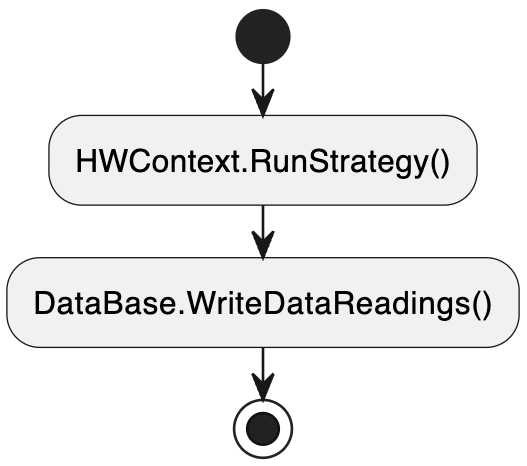
\includegraphics[width=0.4\textwidth]{ReadingJobExecute.png}
    \end{center}
    \vspace{-0.5cm}
    \caption{}
    \label{fig:ReadingJobExecute}
  \end{wrapfigure}
Die \textit{ReadingJob}-Klasse referenziert die Verzeichnise \textit{HM.HWServices} und \textit{HM.DBServices}. Hierbei werden im Konstruktor der Klasse Datenbank so wie Auswertestrategie (Siehe \ref{sec:AuslesenHardware}) instanziiert. Abhängig von Konfigurationsdatei werden hierbei der Name der Datenbank und Auswertestrategie festgelegt. Anschließend werden die benötigten Befehle zum Auslesen und Speichern der Sensordaten, in der Execute Funktion aufgerufen. Diese wird nach ablaufen der \textit{Timer} Zeit aufgerufen. Der Ablaufplan für die Exceute Funktion wird in Abbildung \ref{fig:ReadingJobExecute} aufgeführt.\\

\textbf{CurrentSystemStatusJob}\\
\begin{wrapfigure}{r}{0.3\textwidth}
    \vspace{-1.2cm}
    \begin{center}
      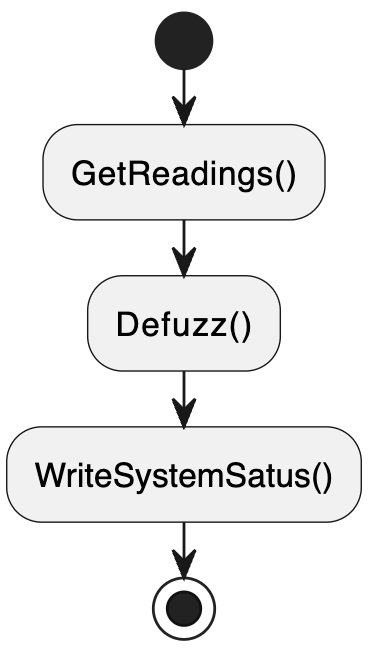
\includegraphics[width=0.3\textwidth]{CurrentSystemStatusExecute.png}
    \end{center}
    \vspace{-0.5cm}
    \caption{}
    \label{fig:CurrentSystemStatusExecuteJobExecute}
  \end{wrapfigure}
Die \textit{CurrentSystemStatusJob}-Klasse referenziert die Verzeichnise \textit{HM.ScoringModel} und \textit{HM.DBServices}. Im Konstruktor der Klasse wird zunächst die Datenbank instanziiert. Anschließend wird abhängig von der In der Konfigurationsdatei hinterlegten Hardwarekonfiguration die Passende \textit{FuzzyLogic}-Klasse geladen (Siehe \ref{fig:ScoringModel}).

